\documentclass[12pt]{article}
\usepackage{ucs}
\usepackage[utf8]{inputenc}
%\usepackage[russian]{babel}
\usepackage{amssymb}
\usepackage[T2A]{fontenc}
\usepackage{amsmath}
\usepackage{amsthm}
\usepackage{amsfonts}
\usepackage{amscd}
\usepackage[alphabetic]{amsrefs}
\usepackage{amsthm}
\usepackage{mathrsfs}
\usepackage{hyperref}
\usepackage{amsmath}
\usepackage{listings}
\usepackage[a4paper,hmargin=0.5cm,vmargin=2.5cm]{geometry}
\usepackage{bbm}
\usepackage{graphicx}
 	
\usepackage{indentfirst} % Красная строка	

\allowdisplaybreaks

\textheight=24cm
\textwidth=16cm
\oddsidemargin=0pt
\topmargin=-1.5cm
\parindent=24pt
\parskip=0pt
\tolerance=2000
\flushbottom
\sloppy


\usepackage{textpos} % package for the positioning
\usepackage{tikz,calc}
\usepackage[english]{babel}



\newcommand{\Cross}{$\mathbin{\tikz [x=1.4ex,y=1.4ex,line width=.2ex, red] \draw (0,0) -- (1,1) (0,1) -- (1,0);}$}%
\newcommand{\Checkmark}{$\color{green}\checkmark$}


\begin{document}
\title{Project Report \\ Low-rank Approximations for Large Incomplete Matrices}
\author{Anton Zhevnerchuk \\ anton.zhevnerchuk@skoltech.ru}
\date{\url{https://github.com/zhevnerchuk/matrix-filling}}

\maketitle

\begin{abstract}
There are some challenging industrial problems in which only incomplete data is available and the goal is to ``complete'' the data. This problem can be stated as an optimization problem in at least two different ways, and a variety of methods can be used for solving the problem in each of the formulations. We implemented three competitive algorithms for matrix-filling problem and compared their performances to each other.
\end{abstract}

\tableofcontents

%------------Background-------------%
\section{Background}

The growth of the Internet influenced the development of recommender systems, data compression and reconstruction. Some of the problems appearing in that fields deal with data, which can be naturally represented as a matrix with some observed values and others values unknown. The goal in such problems is to guess the data at not observed entries. Usually it is assumed that our data has low-rank structure: this assumption follows naturally from the data structure or from the algorithms used for data compression.

%The mutual property of these systems is that all of them deal with data: recommendation systems find the most relevant information for user, storage systems compress files for more efficient capacity using, data reconstruction systems try to find any dependencies in data, to recover it. All the problems occurred in those cases are naturally organized in matrix form. It is worth to mention that there is a considerable number of other areas where partially observed matrix appears, thus it is very important to have accurate and fast algorithms to reconstruct them.

%%%%%%%----------Problem Formulation------%%%%%%
\section{Problem formulation}

We have a matrix $X \in \mathbb{R}^{m \times n}$ with some unknown entries. Let us denote by $\Omega$ the set of positions $(i, j)$ for which $X_{i,j}$ is known. We want to construct a low-rank approximation $Z$ of $X$. In our project we considered two approaches to solving that problem:
\begin{itemize}
\item Fix rank of an approximation and minimize error at known entries;
\item Fix acceptable error at known entries and minimize rank of an approximation.
\end{itemize}

For the following we need to introduce some notation. For a $m \times n$ matrix $A$ $P_{\Omega}(A)$ is a projection of $A$ on the set of known entries:
\begin{align*}
P_{\Omega}(A)_{i,j} = \begin{cases}
A_{i, j}, & (i, j) \in \Omega \\
0, & (i, j) \not\in \Omega
\end{cases}
\end{align*}

When we fix acceptable error at observed entries $\delta > 0$ and minimize rank of an approximation, we have the following problem:
\begin{align}\label{eq1}
\text{minimize} \quad \text{rank}(Z) \qquad \text{subject to} \quad \sum \limits_{(i, j) \in \Omega} (X_{i, j} - Z_{i, j})^2 \leq \delta.
\end{align}
Since this optimization problem \ref{eq1} becomes too hard in general case, the following modification is considered:
\begin{align}\label{eq2}
\text{minimize} \quad \| Z \|_{\ast} \qquad \text{subject to} \quad \sum \limits_{(i, j) \in \Omega} (X_{i, j} - Z_{i, j})^2 \leq \delta.
\end{align}
Here $\| \cdot \|_{\ast}$ is a nuclear norm, which is just a sum of singular values of a matrix. Such a relaxation is a classic approach for matrix-filling problem and is used in many papers (Fazel, 2002; Candes and Recht, 2008; Candes and Tao, 2009; Recht et al., 2007). It occurs that problem \ref{eq2} is convex, which makes it much easier to solve. Nuclear norm is clearly connected with the rank, so in general a solution for \ref{eq2} seems to be also a rather good solution for \ref{eq1}. It can be shown that for every $\delta > 0$ there is a $\lambda > 0$ such that \ref{eq2} is equal to  
\begin{align}\label{eq3}
\text{minimize} \quad \frac{1}{2} \sum \limits_{(i, j) \in \Omega} (X_{i, j} - Z_{i, j})^2 + \lambda \| Z \|_{\ast}.
\end{align}
So, our goal is to solve problem \ref{eq3}. The implemented algorithm (Soft-Input) corresponds to that formulation of a matrix completion problem.

%%%---------Implemented Approaches--------%%%
\section{Implemented approaches}

%%%---------Soft Input--------------%%%
\subsection{Soft-Input}
This algorithm is designed for solving matrix-completion problem in the formulation \ref{eq3}. If all matrix $X$ is known, a solution for \ref{eq3} can be found analytically. If $X = U \Lambda V^T$ is SVD for $X$, a solution is given by
\begin{align*}
Z = U \Lambda_{\lambda} V^T, \, \text{where} \, \Lambda_{\lambda} = \mathrm{diag}\Big(\max\{\sigma_1 - \lambda, 0\}, \dots, \max\{\sigma_{\min\{m, n\}} - \lambda, 0\}\Big).
\end{align*}
Soft-Input is an iterative method for solving \ref{eq3} in general setting with very simple main idea: at each iteration we replace unknown entries of $X$ with the values of a current approximation $Z_\ell$ and solve problem \ref{eq3} for a matrix with all entries known. In \cite{1} it is shown that this iterative algorithm converges to a solution for \ref{eq3}. 

At each iteration we need to find SVD of $m \times n$ matrix $P_{\Omega}(X) - P_{\Omega}(Z_\ell) + Z_\ell$. Note that $Z_\ell$ is a matrix with low-rank, so MATVEC operations can be done in $O((m + n) k)$ flops, where $k$ is rank of $Z_\ell$. Matrix $P_{\Omega}(X) - P_{\Omega}(Z_\ell)$ is sparse. Therefore, if $X$ has good sparse structure, MATVEC operations with matrix $P_{\Omega}(X) - P_{\Omega}(Z_\ell)$ are comparatively cheap as well, so truncated SVD of $P_{\Omega}(X) - P_{\Omega}(Z_\ell) + Z_\ell$ can be found much faster than in general case.


%%%----------Comparative Analysis---------%%%

\section{Demonstration}

We download a photo of one of the buildings in Mendeleev Quarter. After that we set only about $5\%$ of pixels to be known and then we try to repair the photo using some of implemented algorithms. We have achieved the following results:
\begin{center}
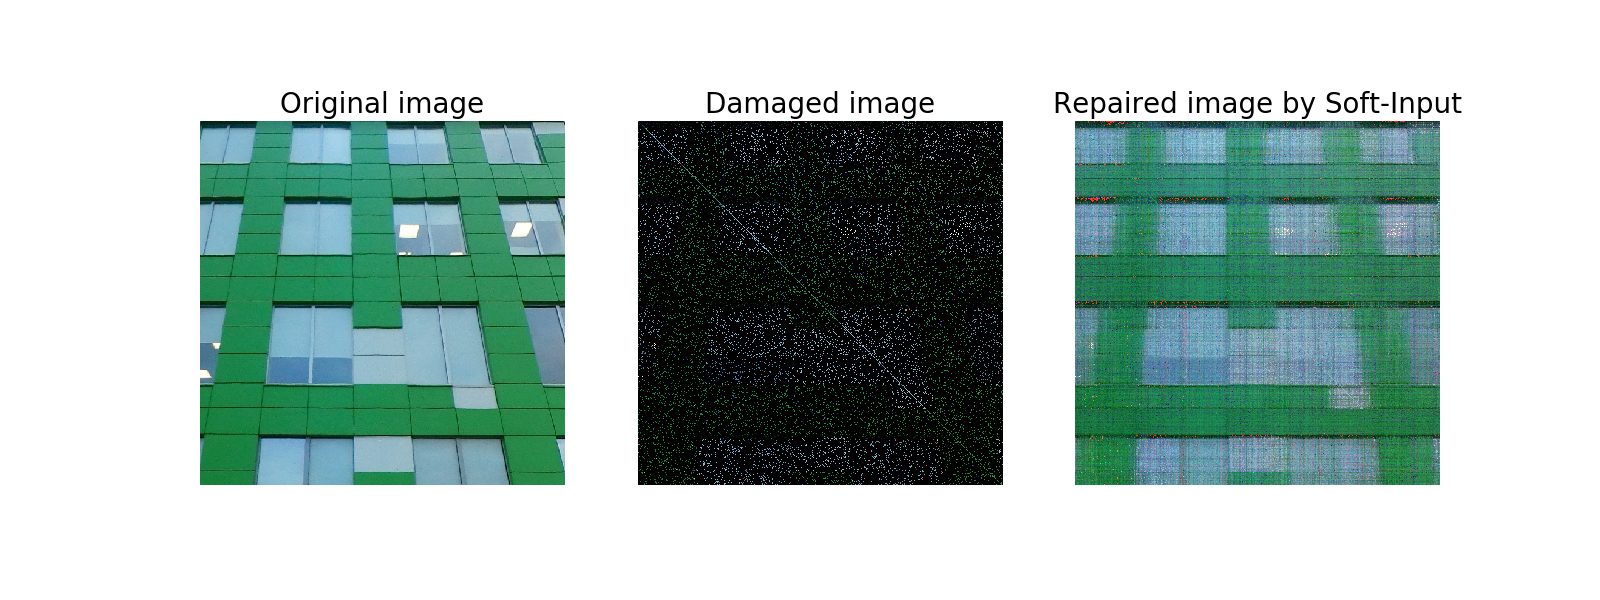
\includegraphics[scale = 0.4]{../Code/demo.png}
\end{center}
We managed to find pretty completion using Soft-Input.

\addcontentsline{toc}{section}{References}
\bibliographystyle{plane}
\begin{bibdiv}
\begin{biblist}

\bib{1}{article}{
    title={Spectral Regularization Algorithms for Learning Large Incomplete Matrices},
    author={Mazumder, Rahul},
    author={Hastie, Trevor},
    author={Tibshirani, Robert},
	journal={Journal of Machine Learning},
    eprint = {https://web.stanford.edu/\%7Ehastie/Papers/mazumder10a.pdf},
    date={2010},
}
\end{biblist}
\end{bibdiv}


\end{document}